\documentclass{article}

\usepackage[nonatbib]{nips_2017}
\usepackage{nips_2017}

\usepackage[utf8]{inputenc} % allow utf-8 input
\usepackage[T1]{fontenc}    % use 8-bit T1 fonts
\usepackage{hyperref}       % hyperlinks
\usepackage{url}            % simple URL typesetting
\usepackage{booktabs}       % professional-quality tables
\usepackage{amsfonts}       % blackboard math symbols
\usepackage{nicefrac}       % compact symbols for 1/2, etc.
\usepackage{microtype}      % microtypography
\usepackage{graphicx}

\usepackage[style=apa,backend=biber]{biblatex}
\addbibresource{NIPS2017.bib}
\DeclareLanguageMapping{english}{american-apa}

\title{Structuring exploration and enhancing learning through intrinsic motivation: A combination of novelty seeking and hierarchical reinforcement learning}

\author{
  Maria K.~Eckstein \\
  Department of Psychology \\
  UC Berkeley \\
  Berkeley, CA 94720 \\
  \texttt{maria.eckstein@berkeley.edu} \\  
  \And
  Tom Griffiths \\
  UC Berkeley \\
  Address \\
  \texttt{tom_griffiths@berkeley.edu} \\
  \And
  Anne GE Collins \\
  UC Berkeley \\
  Address \\
  \texttt{annecollins@berkeley.edu} \\
}

\begin{document}

\maketitle

\begin{abstract}
    Humans have the astonishing ability to learn meaningful behavior from few and unorganized samples, in an environment of sparse rewards, and to create goal-directed action plans in novel, unseen situations, with incredibly quick computation times. All of this has been difficult for artificial intelligence. 


  We propose an algorithm that combines curiosity (intrinsic motivation to explore novel states) and temporal abstraction (creation of option policies at multiple levels of abstraction), with the aim of shedding some light on how structured, goal-directed behavior can arise in complex environment that are sparse in rewards, as shown by humans. The algorithm shows meaningful behavior when exploring a complex environment. The eventual goal is to bring it to humans and see if they do something similar and look into their brains.
\end{abstract}


\section{Introduction}

Humans have the astonishing ability to learn from few and unorganized samples in an environment of sparse rewards, and to create goal-directed action plans in novel, unseen situations, with incredibly quick computation times. How is this possible? Here, we take inspiration from cognitive science and neuroscience to propose a mechanism.

Research in the cognitive sciences over the past decades has suggested that at least two components are crucial for such behavior: hierarchical structure of the representation of the environment or task at hand (Anderson, Collins, Chess study, Miller \& Cohen, 2001, Badre \& Frank); and intelligent exploration, driven by intrinsic motivation and targeted hypothesis testing (Gopnik, Lombrozo, Schmidhuber, painting paper, Deepak's citations). Neuroscience literature shows that novelty is an important driver of exploration, with novel events triggering reward-like signals in the brain [cite DA and novelty literature].

We argue that these two components - intrinsically-motivated exploration and hierarchical representation - are more closely related than is usually acknowledged. Implemented jointly, they can lead to an understanding of the environment that goes beyond and is more flexible than the mere prediction of reward as in traditional RL frameworks (Sutton \& Barto). We argue that by combining intrinsically-motivated exploration with hierarchy, agents can discover meaningful patterns of behavior without explicit training, and learn to form multi-step plans without the need of a predictive model.

We propose a novelty-based hierarchical reinforcement learning (NHRL) algorithm that explores a rewards-free environment based on its intrinsic curiosity, which is triggered by novel events. Once an event triggers the agent's curiosity (imagine an infant playing with a toy that suddenly makes a new sound), the agent will try to reproduce the event (try to reproduce the sound). Crucially, the agent does not know yet how to produce the event that it is curious about. In order to achieve its goal, it therefore has to learn, through trial and error, a specific option policy that leads to the event. In this way, the agent will learn policies to control various aspects of its environment. We model the process of option creation through hierarchical reinforcement learning, relying on the options framework (Sutton, Precup, Singh). Crucially, the only learning signals are fully internally determined: 1) for learning option policies, the agent's internal pseudo-reward upon achieving its self-selected goal; and 2) the events' novelty for learning the value of options.

We show that option policies become better and better at producing their goal events, such that the corresponding events can be produced more frequently and, over time, decrease in novelty. This leads to a decrease in the agent's curiosity, and its intrinsic motivation to explore events further once they are understood. Nevertheless, the world is full of wonders. Whereas an infant might be curious about individual sounds, a toddler might be interested in children's songs, and an adult in twelve-tone music or Italian Opera. Acquiring new skills, rather than reducing motivation and slowing down exploration, opens up new possibilities of learning even more abstract skills. In our framework, basic actions are the building blocks for only the most fundamental option policies. More abstract option policies can be created by using option policies as the building blocks; this process can be repeated indefinitely, resulting in option policies of increasing abstraction, limited only by the temporal horizon of the agent. In other words, the agent can learn to achieve abstract goals by breaking them down into sub-goals and sub-sub-goals, etc.

\section{Methods}
 
\subsection{The task: States, actions, and transitions}

We created a learning environment with a hierarchical structure, as found in more naturalistic circumstances such as language or motor learning, which could be realistically be presented to human learners in future experiments. %Language learning, for example, progresses from learning phonemes to combining phonemes into syllables, syllables into words, words into phrases, phrases into sentences, etc.
In our task, an agent can execute a small number of "basic" actions that trigger specific events in the environment. Each basic action deterministically produces a unique corresponding "basic" (level-0) event. In addition, certain sequences of basic actions trigger a "level-1" event, in addition to the basic event. Similarly, certain sequences of level-1 events produce level-2 events, etc.

Formally, we define $A_0 = a_{0, 1}, a_{0, 2}, \ldots, a_{0, k}$, the set of the agent's $k$ basic actions and $S = {(f_{0, 1}, \ldots, f_{0, k_0}, f_{1, 1}, \ldots, f_{1, k_1}, \ldots, f_{l, 1}, \ldots, f_{L, k_L})}$, the state space defined by binary features $f_{l, i}$ referring to level $l$ and index $i$. The environment's transition function has the following properties. First, if the agent selects $a_{0,i}$ at trial $t$, then the new state's level-0 features are $f_{0,i}=1$ and $\forall j \neq i, f_{0,j}=0$: action $a_{0, i}$ changes the feature $f_{0, i}$ from 0 to 1 - this change in feature is "event" $e_{0, i}$). Second, at any level $l$, there is at most one index $i$ such that $f_{l,i}=1$. To achieve this, all features $f_{l, j}, \forall j$ are set to 0 before feature $f_{l, i}$ is set to 1. Third, at each level $l$, there exist triplets $i \neq j$ and $k$ such that if $f_{l,i}(t)=1$ and $a(t)=a_{l,j}$, then $f_{l+1, k}=1$: lower-level actions in specific states can trigger higher-level events, in addition to their own level's event.

%By defining features this way, the environment has the Markov property even though its workings are defined by sequences of events at varying time scales. 

\subsection{Event novelty and curiosity}

We assume that the agent explores the environment based on its intrinsic curiosity. Curiosity is determined by event novelty and determines the agent's propensity to select an event as a target of exploration, i.e., to set the sub-goal of reproducing the event.

Formally, novelty of event $e$ is defined as $n_e = e^{-\lambda i_e}$ where $i_e$ is the number times event $e$ has occurred since the agent's first encounter with the environment and $\lambda$ is the agent's rate of novelty decay. We assume that curiosity $c_e$ about an event is learned through reinforcement, with delay-discounted novelty serving as a teaching signal: $c_e(t+1) = c_e(t) + \alpha (\gamma^{j_e} n_e(t) - c_e(t))$ whenever event $e$ occurs. Here, $\alpha$ is the agent's learning rate; $\gamma$ is the agent's discounting of the future, and $j_e$ is the number of time steps spent within option $o_e$, which led to event $e$ ($j_e = 0$ when event $e$ happened without executing option $o_e$; $j_e = 1$ when $e$ is a basic event). In order to select specific events as sub-goals, the agent uses $\epsilon$-greedy selection based on its curiosity.

\subsection{Option creation}

Initially, the agent possesses only "basic actions", i.e., it can only select basic events as sub-goals. When a higher-level event occurs for the first time, it is added to the agent's option space as a potential sub-goal. The option policy of the new sub-goal can use all options at the level below to reach the new sub-goal.

Formally, the agent's initial option space $O$ comprises only basic actions, $O = A_0$. When event $e_{l, i}$ occurs for the first time, the agent's option space is extended by the option $o_{e_{l, i}}$ targeted at producing event $e_{l, i}$: $O = O \cup o_{e_{l, i}}$. Option $o_e$'s initiation space is the whole state space $S$; $I$ terminates with probability $p=1$ for all states in which $f_e = 1$ (in which the target event $e$ occurred) and $p = \epsilon_T$ in all other states. The action space of $l$th level option $o_{e_{l, i}}$ comprises all options $o_{e_{l-1, .}}$ at level $l-1$. For example, the policy of a level-1 option $o_1$ operates on the action space comprising all basic actions $a_{0, i} \in A_0$. 

\subsection{Learning option policies}

When the agent selects a specific event $e$ as sub-goal, the option policy $o_e$ controls action selection until the option terminates (see above). The option policy learns through temporal-difference learning (\cite{sutton_reinforcement_2017}) which actions lead to the sub-goal. After the termination of an option, the agent's curiosity about the sub-goal is updated based on the novelty of the produced event (or the failure to produce the event).

Formally, option $o$'s policy $\pi_o$ is $\epsilon$-greedy over within-option values $V_o$. $V_o$ are defined by the weights $\theta$ of the binary features $f(t)$ that describe the state of the environment at time $t$, $V_o^{t+1}(s_t, a_t) = \theta^T f(t)$. 
$V_o$ are updated through temporal difference learning on the weights $\theta$: $\theta(t+1) = \theta(t) + \alpha (r_p + \gamma max_a(V_o^{t}(s_{t+1}, a)) - V_o^{t}(s_t, a_t))$; here, the pseudo-reward $r_p = 1$ when $e$ occurred (and the option terminates) and $r_p = 0$ otherwise; $V_o(s_{t+1},.) = 0$ when the option terminates. 

\subsection{Simulations and competing algorithms} \label{Comparison agents}

We simulated the agents' behavior over environments designed to be sufficiently complex to challenge learning: 5 hierarchical levels ($L = 5$); and $k = 5$ possible events at each level. All rules controlling the occurrence of higher-level events had length 2, i.e., two subsequent events at one level could create an event at the level above.%; rules were allowed to overlap, but could not be identical, e.g., when one rule was $e_{l_2} + e_{l_3} \rightarrow e_{l+1, 1}$ ($e_{l_2}$ followed by $e_{l_3}$ produces $e_{l+1, 1}$), another rule might be $e_{l_2} + e_{l_4} \rightarrow e_{l+1, 2}$). 

Agents were allowed to explore the environment for 400 (section \ref{Results NHRL}) or 300 time steps (section \ref{Results compare all}), i.e., executing 300 basic actions. We used the following parameter settings for all agents: $\alpha = 0.3$, $\lambda = 0.3$, $\gamma = 0.9$, $\epsilon = 0.2$, and $\epsilon_T = 0.1$. We obtain similar results with different parameter sets. The data shown below are based on the average performance of 15 agents in a single environment (section \ref{Results NHRL}), and the average performance of 3 agents in 15 environments (section \ref{Results compare all}). The results hold for individual agents and environments.

To investigate the importance of both hierarchical structure and novelty seeking to behavior, we compared the NHRL agent to three other agents without one or both of these mechanisms. The reward-based hierarchical agent created and employed options in the same way as the NHRL agent, but used reward $r$ instead of novelty as an update signal for option values; we define reward as the number of events produced in a given trial.
The novelty-based flat agent selected options based on curiosity like the NHRL agent, but it did not create or use options. Therefore, $O = A_0$ and $S = S_0$. The reward-based flat agent is a combination of these two agents, with neither options nor novelty-based learning.


\section{Results}

\subsection{Behavior of the NHRL agent} \label{Results NHRL}

Through exploration and experience of novel events, the NHRL agent acquired several different, hierarchically structured option policies. Thereby, option policies targeted at simpler events were learned faster than for complex events, and final policies were also more accurate (data not shown).

In addition, as expected, the agent's curiosity decreased fastest for basic events (level 0), and slower for events at higher levels of abstraction (levels 1-4) (fig. \ref{CuriosityFigure}). In other words, the simpler an option, the faster the agent lost interest in executing it for it's own sake. Importantly, this does not imply that the agent executed simple options less often overall. On the contrary, the rate of all abstract events increased over time (see fig. \ref{CEvents}). The reason for this is that simple options form the building blocks of all abstract options.

%Finally, the agent showed some kind of "specialization": The higher the level of abstraction, the fewer events it discovered. The reason for this is that once a higher-level option is discovers, it dominates behavior and less exploration
%level-1 events required the sequential execution of two specific level-0 actions, whereas level-4 events required the sequential occurrence of 2 level-3 events, which correspond to 4 level-2 events, and eventually 16 basic actions. 

\begin{figure}[h]
	\centering
	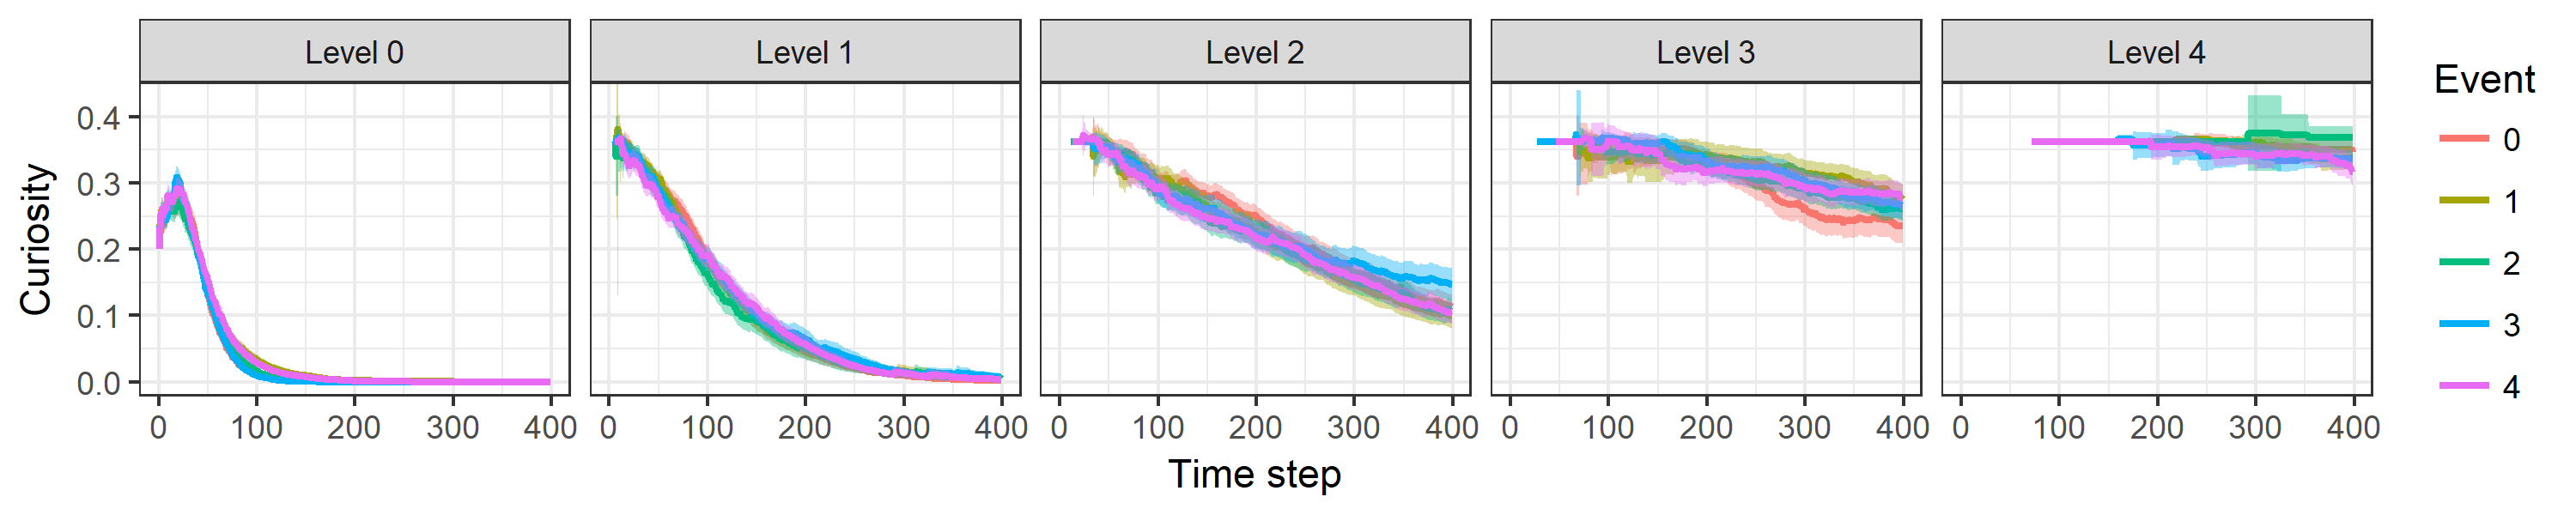
\includegraphics[width=\linewidth]{ACuriosity.png}
	\caption{Curiosity for events decreases over time. Shaded areas indicate the standard error of the mean. The higher-level an event, the slower curiosity decreases. The environment contained 5 different events at each level of abstraction. The agent does not usually discover all events (e.g., only one event was discovered at level 4.)}
	\label{CuriosityFigure}
\end{figure}

\subsection{Comparison of the NHRL agent and other agents} \label{Results compare all}

We finally compared the behavior of the NHRL agent to three other three agents (see section \ref{Comparison agents}). The NHRL agent discovered a larger number of different events than any other algorithm, and at a faster rate (fig. \ref{CEvents} A). Both the novelty-based flat agent and the reward-based hierarchical agent outperformed the reward-based flat agent, suggesting that both curiosity and hierarchical structure were crucial for effective exploration.

The reason for the exploration advantage is the NHRL agent's specific pattern of curiosity, with larger curiosity for higher-level events. Due to that, the agent will execute more higher-level options (fig. \ref{CEvents} B), which increases the probability of observing events at higher levels. 

\begin{figure}[h]
	\centering
	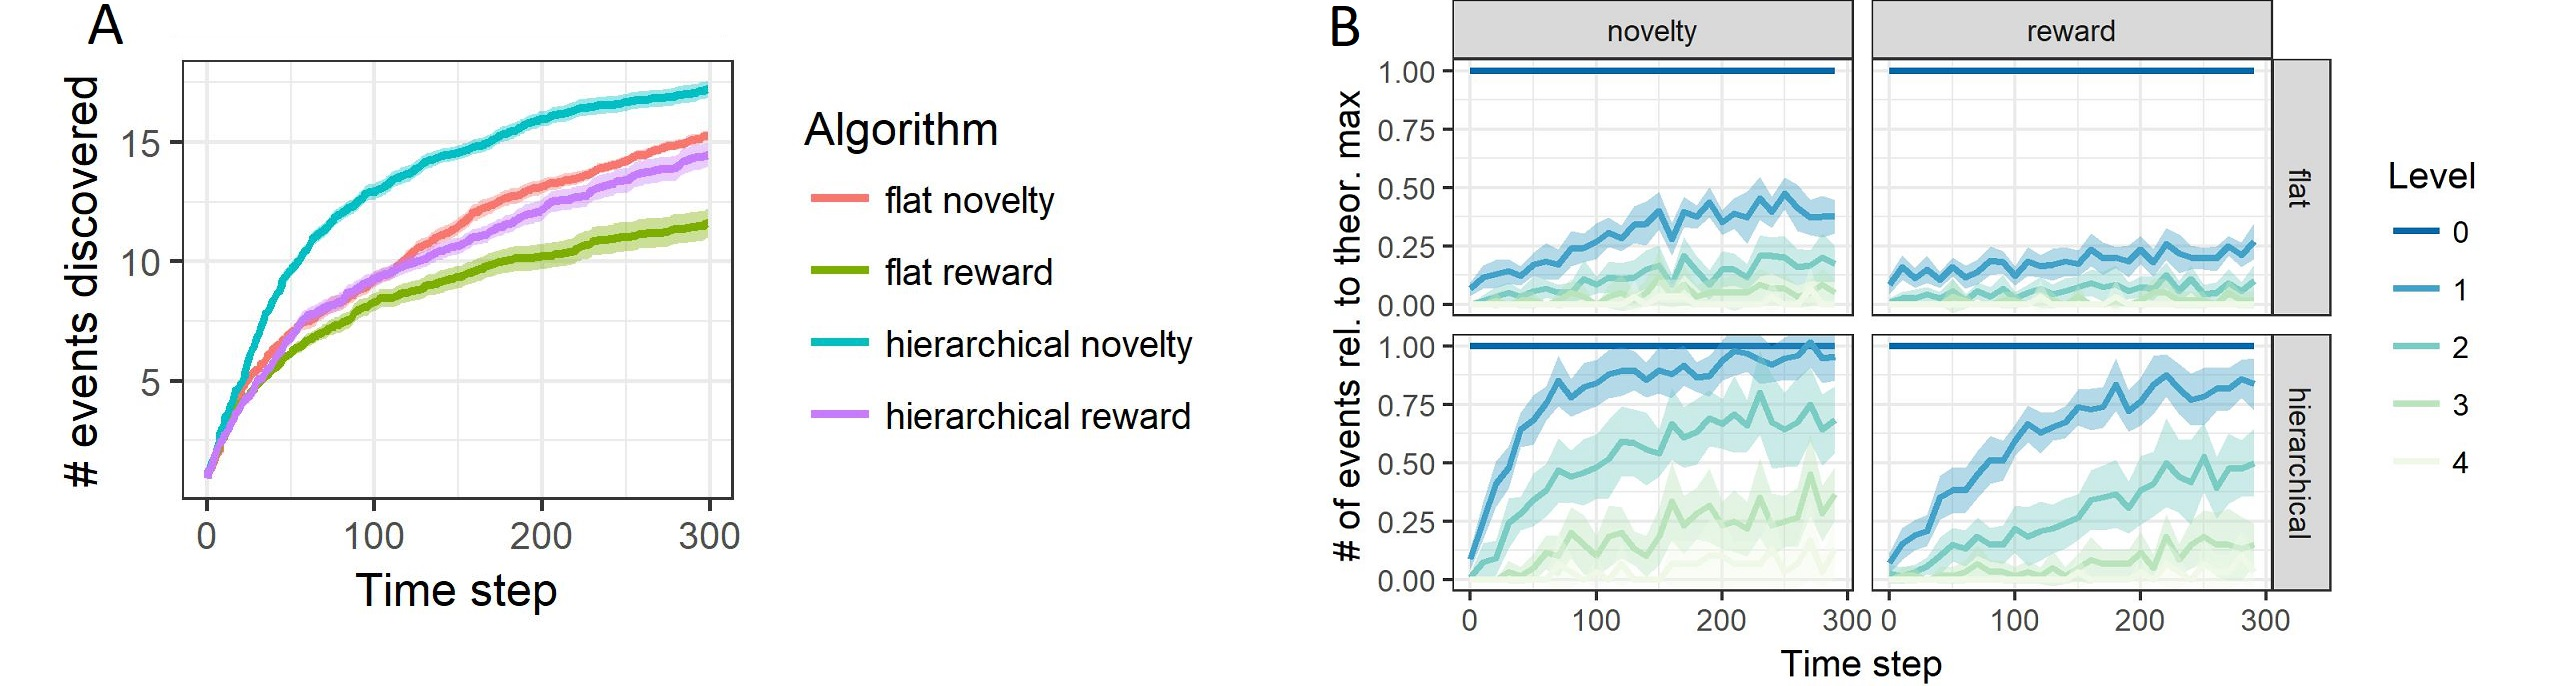
\includegraphics[width=\linewidth]{CEvents.jpg}
	\caption{A) Number of events discovered by each of the four agents over the course of 300 time steps. B) Number of events that occurred in each bin of 10 time steps, relative to theoretical maximum (theor. max. for level-0: 10 / 10; level-1: 5 / 10; level-2: 2.5 / 10; etc.). Shaded areas indicate 95\%-confidence interval of the mean.}
	\label{CEvents}
\end{figure}


\section{Conclusion}

We have shown that a NHRL agent explores an environment with hierarchical structure in a more goal-directed and thorough way than a flat agent. It discovers more different events and learns strategy to reproduce these events at iths own wish. Doing this, it does not get bored - very simple action sequences (options) get boring, but it keeps adding abstract goals, which get less and less boring. 

This makes sense and might be similar to humans.

The agent learns to "understand" its environment. It is able to predict events and control them according to its own wishes.

This is interesting because usually people think about prediction in terms of model-based (versus model-free) methods, rather than hierarchical methods. But creating hierarchy in this way really is a way to achieve prediction. By creating an event option policy, the agent learns to predict the event. By selecting the option policy, it controls the environment.

"Embodiment" is really important, the possibility of the agent to interact with its environment. Because understanding implies control. Kids love to experiment. Cite stuff on how experimentation helps kids learn? (Fei Shu, Tania Lombrozo?, Alison Gopnik?; active learning literature)

Der algo ist auch weniger fehleranfaellig: Er kann bestimmte Fehler machen und trotzdem das higher-level event erreichen. Eine Form of generalizing.

%Because options are strictly hierarchical in this way, time scales differ between options at different levels. Level-1 option policies are updated at each time step (because the agent executes one basic action at each time step), but level-2 option policies are only updated after a chosen level-1 option terminates. In the experiments presented below, all events are triggered by the sequential occurrence of two events at the level below. Therefore level-2 option policies can at most be updated every other time step, level-3 options every fourth, level-4 option every 8th, and so on.
 %Related work has suggested that this is a valuable approach (Work on novelty: Deepak Pathak, Pulkit Arawal, Yael Niv, Schmidhuber; on hierarchy: Marlos Machado, Botvinick, Yael Niv, Pedro Tsividis; combination of both: Deep HRL paper)

\subsection{Future directions}

\begin{itemize}
	\item Algo itself could be extended: function approximation (neural network) rather than tabular RL; model curiosity in a more sophisticated way: based on prediction rather than event count (Deepak Pathak's citations)
	\item Bring the task to humans and compare
	\item extract RL features and look for them in the brain
	\item Check if we can reproduce specific phenomena related to hierarchical learning. First, does the agent have a learning advantage when it is allowed to explore the environment first (without rewards), before asked to exploit it (add rewards, see how long it takes the agent to find the best strategy, compared to a flat or non-trained agent). Second, is there interference when the agent is trained in one environment and then posed into an environment whose options are just slightly different (reason why second-language speakers never get rid of their accent: it's situated at a low level in the language hierarchy).
	\item Check if there is more on the powerpoint.
	\item Maybe all is really just exploration: Science, in the end, is the task of understanding the world.
\end{itemize}

Taken together, by creating the hierarchical novelty-seeking agent, we hope to show that learning of meaningful behavior can be driven by learning itself, rather than external rewards. In this framework, the learner produces the crucial learning signals itself, by selecting actions that over time reduce novelty. In other words, this learner balances the search for novelty with reducing prediction errors. It explores the environment in a systematic way, forms "hypotheses" and conducts "experiments", in order to learn more. 

\if 0
\subsection{Old Intro}

It is desirable for a complex cognitive system, like a human, to understand its environment in a way that allows prediction of future states and events. This is because with the ability to predict the results of its own actions, an agent will be able to control its environment, creating the states and events it desires. The prediction and control of future rewards, for example, has been formalized in reinforcement learning theory (\cite{sutton_reinforcement_2017}). In this framework, an agent learns over time how much (cumulative, temporally discounted) reward to expect in the future, given the current state of the environment and the agent's action policy. Given the ability to predict, the agent can then maximize future rewards by adjusting its action policy.

\begin{itemize}
	\item But it's not all about rewards: We want to learn the structure of the environment (predictive model) before we know which states and actions will be rewarding.
	\item Example: When an infant looks at a computer monitor, she probably sees a dark frame, filled with colored rectangles and blinking, moving blobs of various sizes. A computer-savy adult, on the other hand, sees a Mac or Windows machine, a bug in the code, or the need to download a new plugin. The perception of the computer monitor changes dramatically upon interaction with it. Interaction creates a structured model of the computer.
	\item Other examples: language learning: learn phonemes, syllables, words, 2-word sentences, 3-word sentences, whole sentences, poetry; motor learning: learn to grasp, hold, manipulate, ..., play the violin.
	\item Indeed, psychological research of the last century has stressed again and again that humans represent their world hierarchically (Chess study - chunking; old research on expertise; TS; Anderson? Making coffee)
	\item What would a predictive model look like that is not focused on reward? Instead of a flat table that specifies how much reward to expect from each state-action pair, we would have a collection of policies that specify how to reach various states in the environment. The agent can control the environment by selecting whatever sub-goal it likes at the moment. Once rewards are added, it can use the learned structure to maximize rewards. 
	\item introduce HRL
	\item ML / RL advances in this direction: Machado, ... (cite papers that talk about exploration; sparse rewards; old 2-step paper; Schmidhuber; Deepak Pathak; the other papers in dropbox papers and in the old draft)
	\item The big question is now how to find valuable sub-goals. Much research, mostly about bottleneck states in the state space (Botvinick -> check in my powerpoint). But this is unrealistic: an agent does not have access to all the information necessary to calculate which states are bottleneck states. 
	\item The goal of this project is to create an algorithm with human-like behavior. Valuable sug-goals will be identified using the agent's curiosity, i.e., intrinsic motivation (Deepak Pathak's citations; Botvinick paper? -> check powerpoint)
\end{itemize}
\fi 

\printbibliography

\end{document}